\chapter{Cryptocurrency Wallets}
\label{ch:wallets}

Traditioneel wordt fysiek geld in een portemonnee bewaard. Voor grotere bedragen verwerken en registreren banken tegenwoordig het digitale saldo van de fiat currency (\$, \pounds, \euro) op een rekening op naam. De algemene consensus is dat men altijd toegang heeft tot het geld en dit op elk gewenst moment kan opnemen. Helaas, vanaf het moment dat het geld op de bank staat, is dit juridisch gezien van de bank. Je hebt een vordering op de bank, dat wel, maar je bent het volledige initiatief en de controle over je eigen geld kwijt. Wanneer je digitale fiat currencies omzet in cryptocurrencies als Bitcoin, kun je geld zo beheren dat alleen jij er toegang toe hebt. En je hebt op elk moment volledige toegang, zonder \emph{counterparty risk} (risico vanuit een tegenpartij). Dit komt simpelweg omdat je van niemand afhankelijk bent en daardoor altijd toegang hebt tot jouw financi{\"e}le middelen. 

\begin{figure}
    \centering
    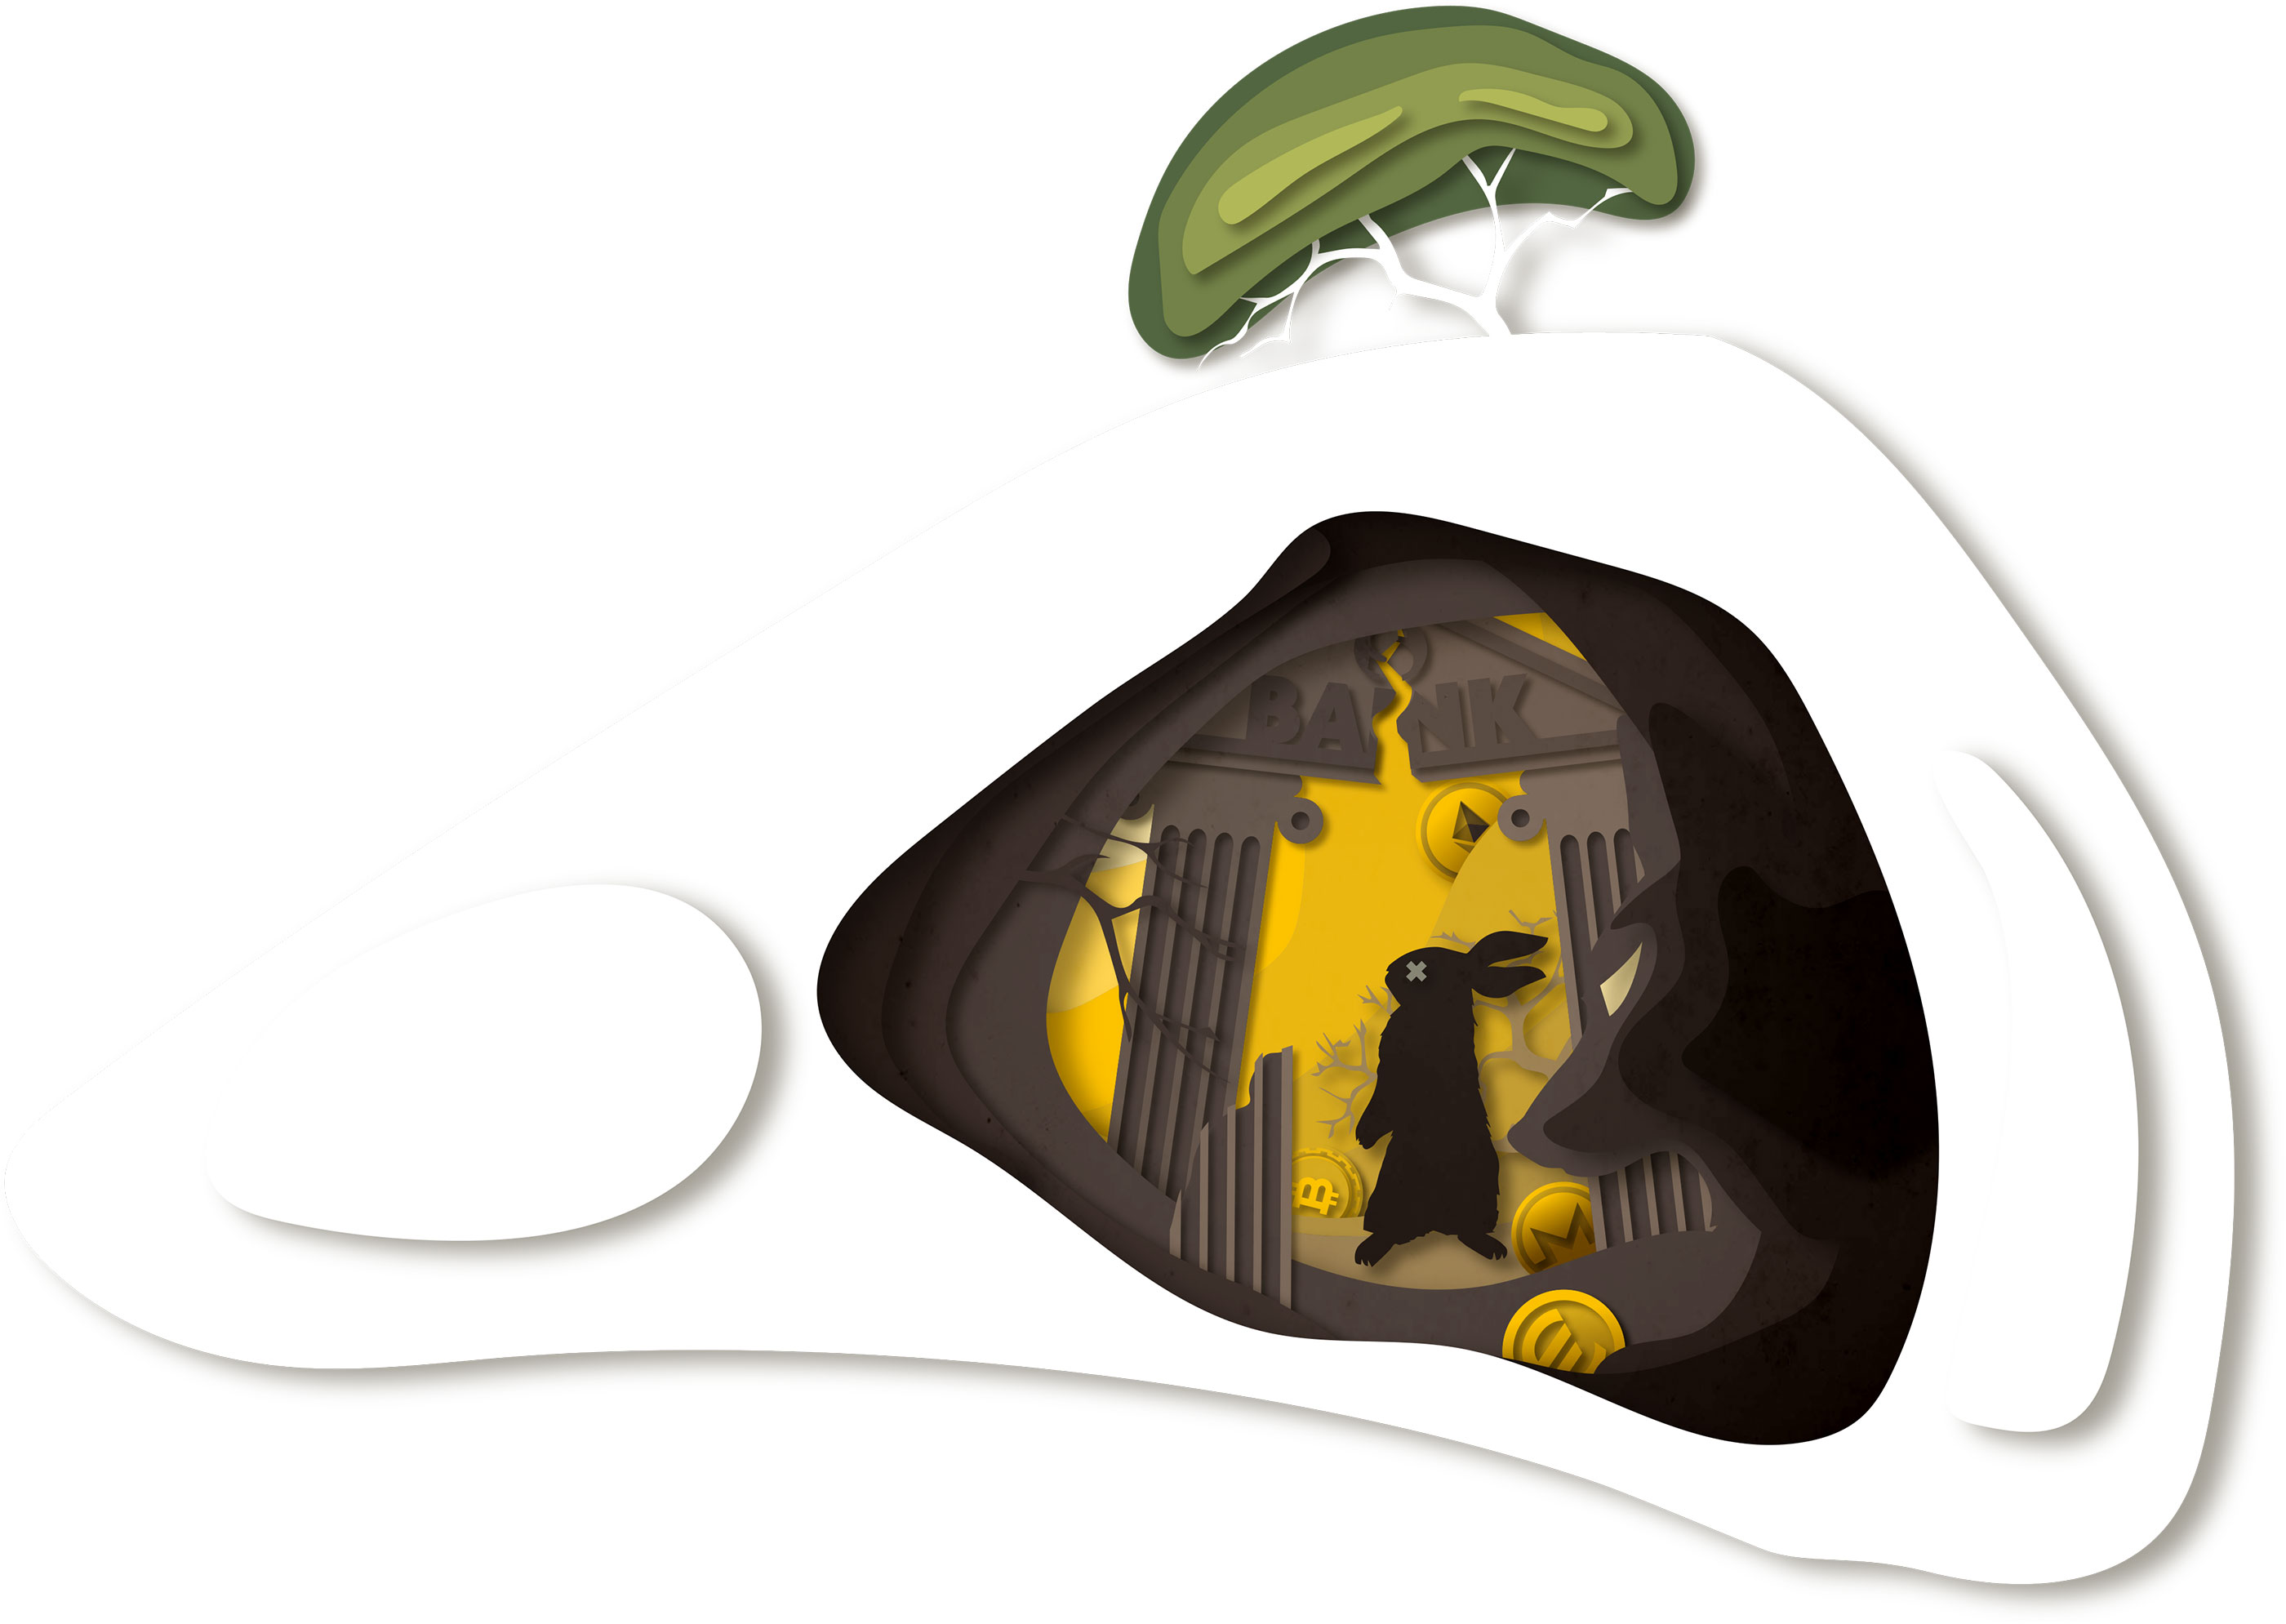
\includegraphics[width=\textwidth]{illustrations/resized_CRYPTO_KEY_1_PART_3.jpg}
\end{figure}

\begin{quotation}

      \textit{\say{Wanneer je geld op de bank zet, wordt de bank wettelijk de eigenaar van dat geld. Met cryptocurrencies ben jij de eigenaar. Als de banken jouw geld bezitten, geven ze het uit zoals ze willen. Als jij het bezit, geef jij het uit zoals jij wil. Cryptocurrency is bestand tegen censuur en niemand beslist of je het wel of niet kunt uitgeven en waaraan}}
      \begin{flushright}
        \small{--- \textbf{Simon Dixon}}
      \end{flushright}
    
\end{quotation}

\section{Wat zijn cryptocurrency wallets}
Cryptocurrency wallets zijn software-programma's die ons in staat stellen met het netwerk - de blockchain - te communiceren. Deze communicatie bestaat uit het versturen en verwerken van transacties op het netwerk. De transacties worden vervolgens uitgevoerd op de blockchain en de balansen worden aangepast en geregistreerd op het netwerk, waarna wallets deze weer kunnen uitlezen. Je kunt een cryptocurrency wallet praktisch gezien vergelijken met een bankrekening, mailbox of een e-mailadres. Je kunt met elk van hen communiceren als je de zogenoemde \emph{public key} weet, een email of bankrekeningnummer bijvoorbeeld. Om aan te tonen dat je eigenaar bent van een bankrekeningnummer of email, gebruik je daarnaast altijd een \emph{private key}, veelal een regulier wachtwoord. Indien je gebruik wilt maken van cryptocurrencies en transacties wilt uitvoeren met die betreffende crypto, heb je een wallet nodig die de specifieke cryptocurrency, of onderliggende platform, ondersteunt en dus jou in staat stelt met het netwerk - de blockchain - te communiceren. Er zijn wallets die meer dan honderden cryptocurrencies ondersteunen.\medskip 

\begin{cryptobox}{PLAY ON THE BLOCKCHAIN}

    \say{Met een cryptocurrency wallet, beheer jij je cryptocurrencies in de vorm van gevalideerde transacties op de blockchain. De wallet genereert en bewaart private keys en public keys, communiceert met het betreffende netwerk - de blockchain - en stelt gebruikers in staat om transacties uit te voeren en te ondertekenen.} \footnote{Ethos (2018); \href{https://www.ethos.io/what-are-cryptocurrency-wallet-private-keys-addresses/}{What are Cryptocurrency Wallets, Private Keys and Addresses}.}
    
\end{cryptobox}

\section{Hoe werken cryptocurrency wallets}
In tegenstelling tot wat vaak wordt gedacht, slaan crypto wallets geen cryptocurrencies op. In plaats daarvan staan ze interactie met de blockchain toe. Met andere woorden, wallets kunnen de nodige informatie genereren om cryptocurrency te versturen en te ontvangen via blockchain transacties.

\subsection{Public \& private key pairs}

Cryptocurrency wallets hebben een publiek adres, een alfanumerieke identificatiecode. Dit adres is gegenereerd op basis van de public en private key. Het adres is eigenlijk een specifieke locatie of \say{tag} op de blockchain waar de crypto naartoe kan worden gestuurd. Dit betekent dat dit publieke adres met anderen gedeeld kan worden om crypto te ontvangen, maar maak de bijbehorende private key nooit aan iemand bekend. Een private key geeft toegang tot de wallet, ongeacht op welk apparaat deze wallet wordt gebruikt. Dus zelfs als de computer of smartphone is gecompromitteerd, is er nog steeds toegang tot de cryptocurrency via een ander apparaat - zolang de corresponderende private key (of \href{https://www.binance.vision/glossary/seed-phrase}{seedphrase}) maar bekend is. Onthoud dat cryptocurrency nooit fysiek verplaatst wordt op de blockchain, ze worden alleen maar af- en bijgeschreven op verschillende adressen, de transacties zijn onomkeerbaar en bij een open blockchain openbaar zichtbaar.

\tikzset{%
  >={Latex[width=2mm,length=2mm]},
  % Specifications for style of nodes:
            base/.style = {rectangle, rounded corners, draw=black, minimum width=4cm, minimum height=1cm, text centered, font=\sffamily},
            privatekey/.style = {base, fill=cryptoorange},
            publickey/.style = {base, fill=cryptogold},
            publicaddress/.style = {base, fill=cryptogreen, font=\sffamily},
            }
            
\begin{figure}[hbp]
  
  \centering
    \begin{tikzpicture}[node distance=2.5cm,every node/.style={fill=white, font=\sffamily}, align=center]
      % Specification of nodes (position, etc.)
      \node (privatekey)       [privatekey]                             {Private Key};
      \node (publickey)        [publickey, below of=privatekey]            {Public Key};
      \node (publicaddress)    [publicaddress, below of=publickey]        {Public Address};
     
      
      \draw[->]             (privatekey) -- node[text width=4cm] {One way hash function(s)} (publickey);
      \draw[->]             (publickey) -- node[text width=4cm] {One way hash function(s)} (publicaddress);
      
      \draw [red, dashed, very thick] (3,-1.25) node {X} (3,-3.75) node {X};
       
      \draw [->,red, dashed, very thick](2,-2.5) .. controls (3,-2.5) and (3,0) .. (2,0);
      \draw [->,red, dashed, very thick](2,-5) .. controls (3,-5) and (3,-2.5) .. (2,-2.5);
        
      \draw [->,green, dashed, very thick](-2,0) .. controls (-3,-0) and (-3,-2.5) .. (-2,-2.5);
      \draw [->,green, dashed, very thick](-2,-2.5) .. controls (-3,-2.5) and (-3,-5) .. (-2,-5);
    \end{tikzpicture}
    \vspace{2mm}
    \caption[Relaties tussen de private key, public key en het publieke adres]{De private key wordt gebruikt om een public key te genereren, wat resulteert in een publiek adres. Het is niet mogelijk om met terugwerkende kracht achter de private of public key te komen.}
    \label{flowchart:keys}
    \source{\emph{Online text \& file hashing. \href{http://www.hashemall.com}{hashemall.com}}}
\end{figure}


\subsection{Hot \& cold wallet}
Wanneer men over wallets leest, worden al snel de termen \say{hot} wallet en \say{cold} wallet gebruikt. Alle verschillende soorten wallets vallen onder {\'e}{\'e}n van deze twee catagori{\"e}n. Over het algemeen is elke wallet die met het internet is verbonden een \say{hot} wallet. Wallets die niet direct in verbinding met internet staan, noemt men \say{cold} wallets, ook wel bekend als \emph{cold storage}. Online, desktop en mobiele wallets zijn altijd hot wallets, terwijl hardware en papieren wallets geclassificeerd worden als cold wallet.

\paragraph{Hot wallet}
Over het algemeen zijn hot wallets gemakkelijk toegankelijk via mobiele apparaten, laptops en desktops. Hier kunnen cryptocurrencies relatief snel, gemakkelijk en via gebruiksvriendelijke interfaces worden beheerd. Het nadeel van hot wallets is dat deze \say{custodial} zijn, wat betekent dat een derde partij de private keys beheerd. Hot wallets zijn zeer handig voor mobiele gebruikers en worden met name gebruikt voor kleine hoeveelheden cryptocurrency. Gebruikers moeten echter nooit grote bedragen in hot wallets opslaan. Behandel deze wallets zoals je een fysieke portemonnee zou behandelen en neem niet teveel crypto's in een keer mee. 
\paragraph{Cold wallet}
Cold wallets zijn de industriestandaard (best practices) voor de veilige opslag van cryptocurrencies. Cold wallets zijn offline wallets en dus niet blootgesteld aan het internet. De meest bekende vormen van cold wallets zijn hardware wallets (\cref{subsec:hardware-wallets}) of paper wallets (\cref{subsec:paper-wallets}). Mede omdat ze volledig offline zijn en de private keys versleuteld en in eigen beheer zijn, zorgen deze cold wallets voor een veel hoger veiligheidsniveau.

\medskip

\section{Verschillende soorten wallets}
Er zijn verschillende soorten wallets waarmee op verschillende manieren cryptocurrencies kunnen worden beheerd. Wallets kunnen onderverdeeld worden in drie verschillende categori{\"e}n: software, hardware, en papieren wallets. 

\medskip

\subsection[Software wallets] {Software wallets (hot)}
Software wallets kunnen functioneren op een desktop, online, of op een mobiel apparaat. Hardware wallets gebruiken hun eigen software, al vallen ze onder de hardware categorie omdat ze uitgevoerd zijn als gespecialiseerde USB-apparaten.

\subsubsection [Desktop wallets]{Desktop wallets}
Desktop wallets bieden volledige controle over keys en crypto. Wanneer je een nieuwe desktop wallet installeerd, wordt een bestand genaamd \say{wallet.dat} lokaal op de computer opgeslagen. Dit bestand bevat de informatie (keys) die wordt gebruikt om toegang te krijgen tot jouw cryptocurrency in die wallet. Elke keer dat de desktop wallet geopend wordt moet het wachtwoord worden ingevoerd, zodat het bestand \say{wallet.dat} kan worden gelezen. Als men dit bestand verliest of het wachtwoord vergeet, verliest men zeer waarschijnlijk de toegang tot de cryptocurrency. 

Daarom is het cruciaal om een back-up te maken van het wallet.dat bestand en dit ergens veilig te bewaren. Men kan ook de corresponderende private en public keys of seedphrase exporteren. Door dit te doen, is men altijd in staat om toegang te krijgen tot de crypto op andere apparaten.

In het algemeen kan een desktop wallet als veiliger worden beschouwd dan de meeste web wallets, maar het is cruciaal om ervoor te zorgen dat de computer schoon is van virussen en malware voordat een desktop wallet in gebruik genomen wordt.\medskip

\begin{borderbox}
    \centering
    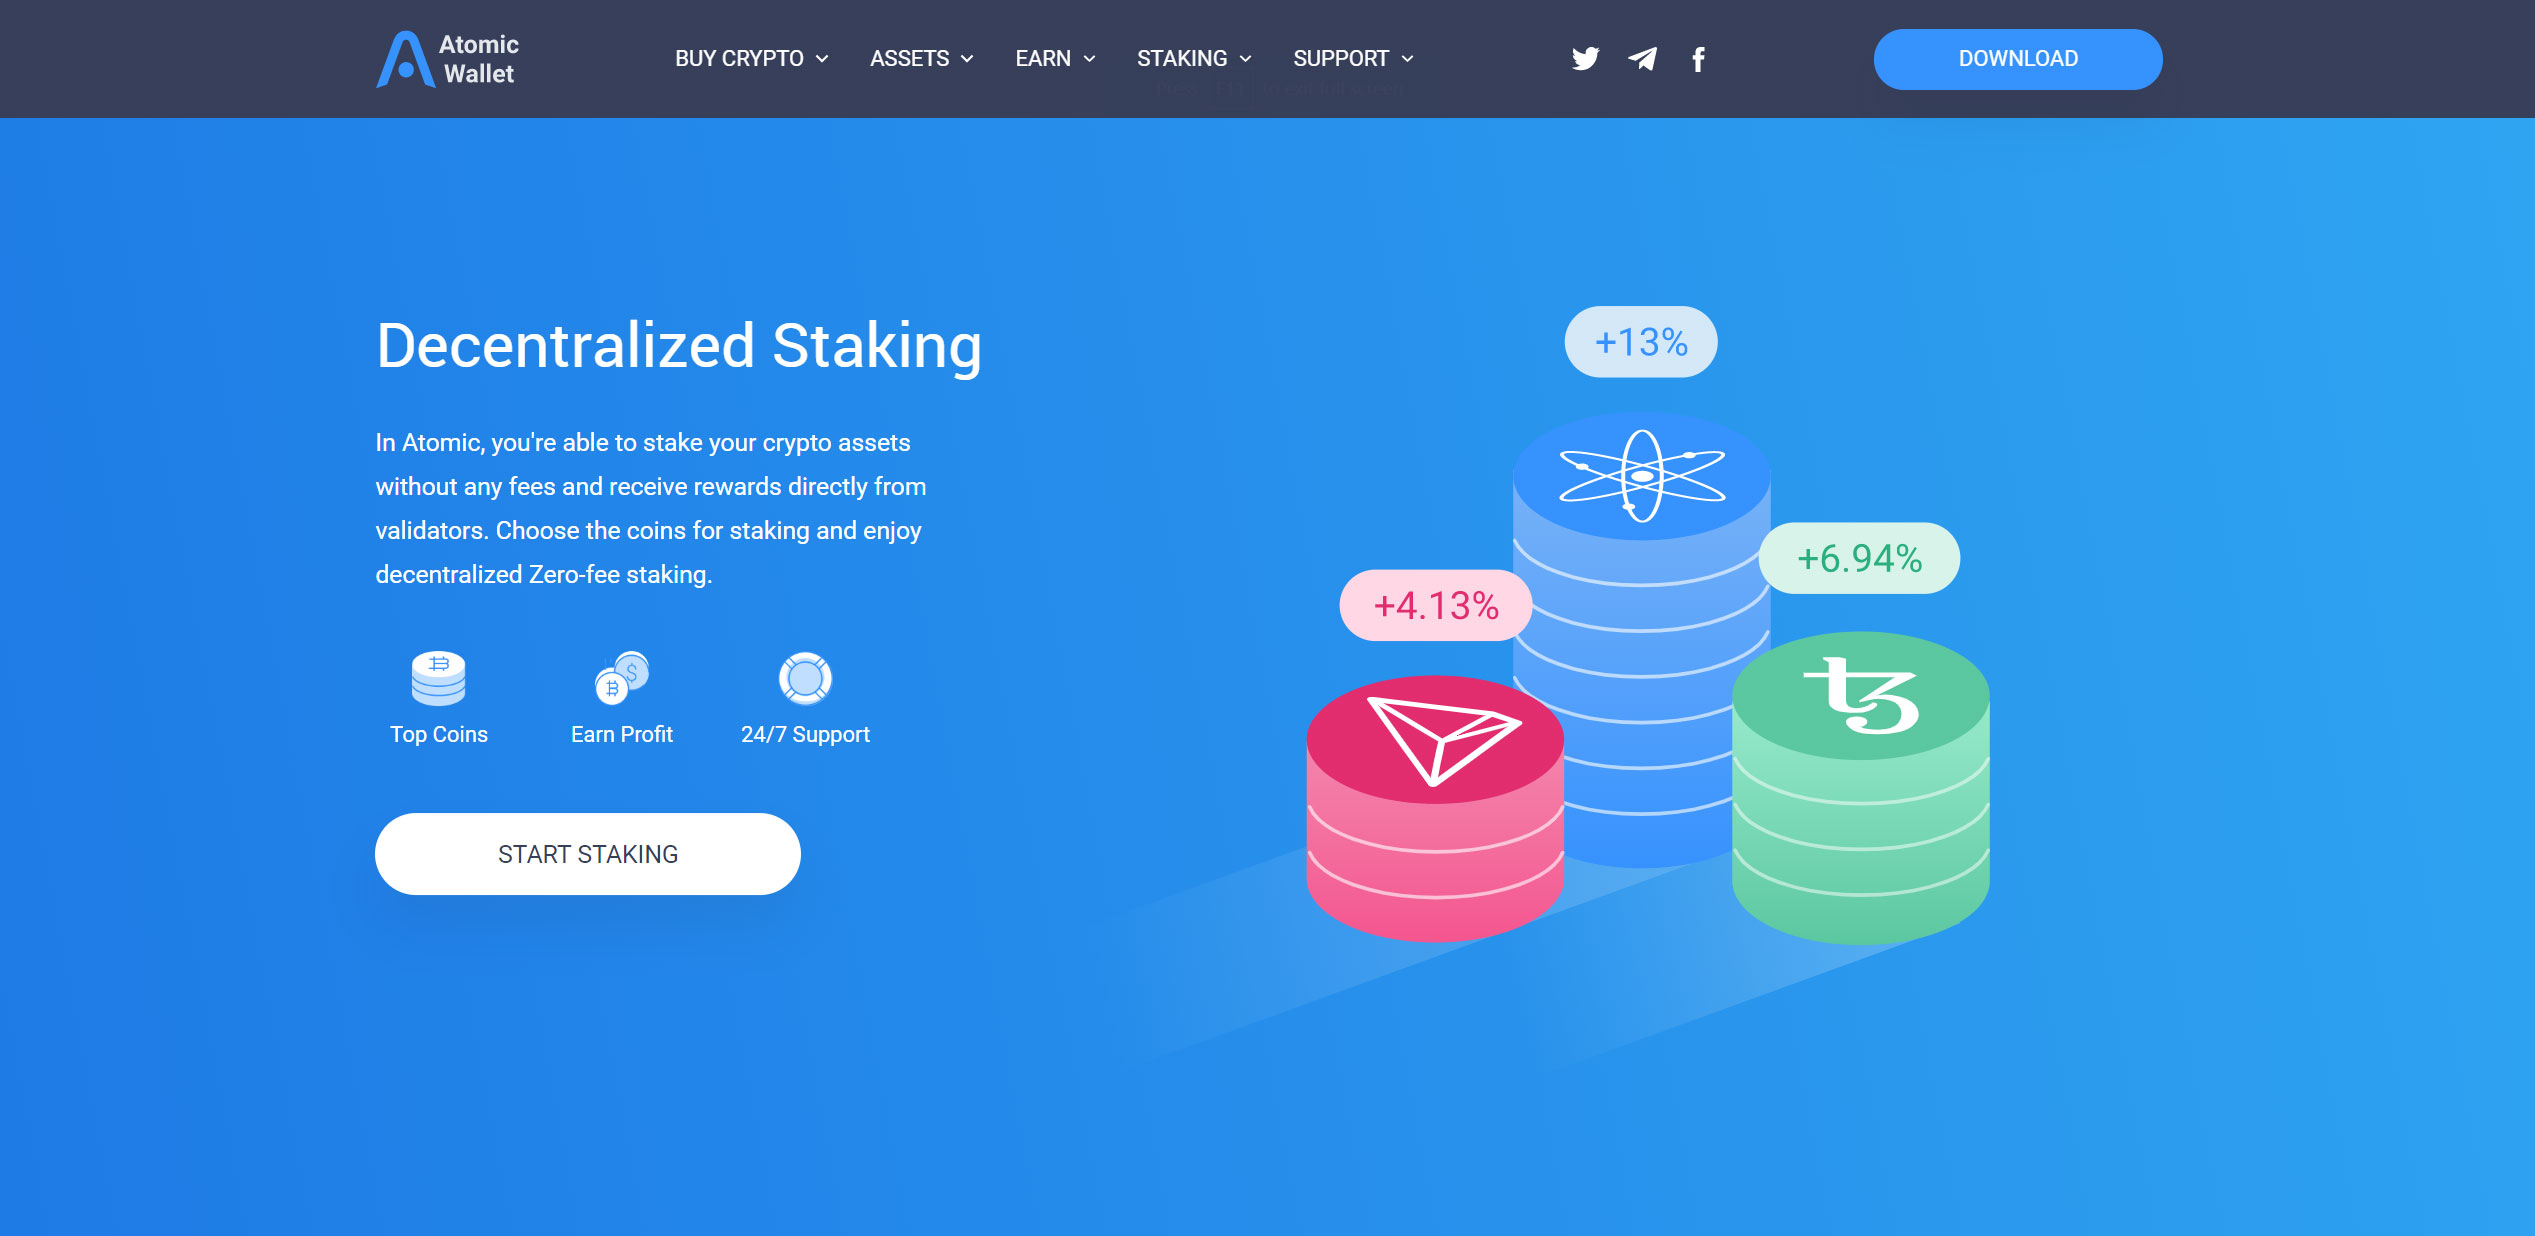
\includegraphics[width=\textwidth]{img/ch-wallets/atomic_wallet1.jpg}
\end{borderbox}
\medskip

\begin{tipbox}{\textbf{Tip}}
 Deze desktop wallets ondersteunen gigantisch veel cryptocurrencies en zijn daarnaast makkelijk te gebruiken. Perfect voor beginners.
\tcblower 
Gebruik bijvoorbeeld \href{https://atomicwallet.io/}{Atomic Wallet} of \href{https://www.exodus.io/}{Exodus Wallet}.
\end{tipbox}\medskip


\subsubsection[Mobiele wallets] {Mobiele wallets} 
Een mobiele wallet is een wallet-applicatie op je telefoon. Ze kunnen overal worden gebruikt en meegenomen dus is het erg handig voor in gebruik. Ze werken net als desktop wallets maar zijn specifiek ontwikkeld voor gebruik op mobiele aparaten en het werken met QR-codes. Voor mobiele wallets geldt tegenwoordig dat ze vrijwel niet meer onder doen voor dekstop wallets op computers, vanwege het grotere scherm blijven veel activiteiten toch prettiger op een computer. 

Mobiele wallets zijn bijzonder geschikt voor het uitvoeren van dagelijkse transacties en betalingen. Ze worden dus hoofdzakelijk gebruikt voor het uitgeven of uitwisselen van Bitcoin en andere cryptocurrencies. 

Net als desktop computers zijn mobiele apparaten ook kwetsbaar voor aanvallen en malware-infecties. Daarom is het aan te raden de mobiele wallet te versleutelen met een wachtwoord en een back-up te maken van de private key. Voor het geval de smartphone verloren of kapot gaat.
Hoe meer het gebruik van cryptocurrency wordt ge{\"i}ntegreerd in het dagelijks leven, hoe meer men gebruik zal maken van mobiele wallets.\medskip

\begin{tipbox}{\textbf{Tip}}
 Deze wallets zijn onmisbaar voor iedereen die altijd en overal toegang nodig heeft tot zijn of haar cryptocurrency.
\tcblower 
Gebruik bijvoorbeeld de \href{https://www.ethos.io/universal-wallet/}{Ethos Universal Wallet}.
\end{tipbox}

\subsubsection[Web wallets]{Web wallets}
Web wallets zijn altijd verbonden met het internet en toegankelijk via verschillende internetbrowsers zoals Brave, Google Chrome, en Firefox. De private keys worden in dit geval online bewaard in de browser zelf.  

Web wallets worden over het algemeen aangeboden door gecentraliseerde cryptocurrency exchanges. Daarnaast zijn er ook web wallets die niet gehost worden en waarbij de gebruiker zelf verantwoordelijk is voor zijn eigen keys. Wij raden altijd aan om \say{non-hosted wallets} te gebruiken indien mogelijk, zodat de cryptocurrency altijd toegankelijk is en in eigen beheer.

\paragraph{Non-hosted wallets}
Voorbeelden van non-hosted wallets zijn \href{https://www.myetherwallet.com}{MyEtherWallet} en \href{https://www.metamask.io}{MetaMask}. Beide stellen ze gebruikers in staat om zelf controle te behouden over de cryptocurrencies en zijn ze daarnaast gemakkelijk te bedienen.

\paragraph{Hosted wallets}
De meest beruchte web wallets zijn de wallets die de verschillende exchanges aanbieden en beheren. Bij een online exchange wallet is de gebruiker niet in het bezit van zijn of haar \emph{private-keys} of \emph{priv{\'e}-sleutels}. Hier beheren de exchanges deze voor de gebruikers, en loggen die in met een gebruikersnaam en een wachtwoord combinatie, die gelinkt zijn aan de keys. 
\medskip

\begin{borderbox}
    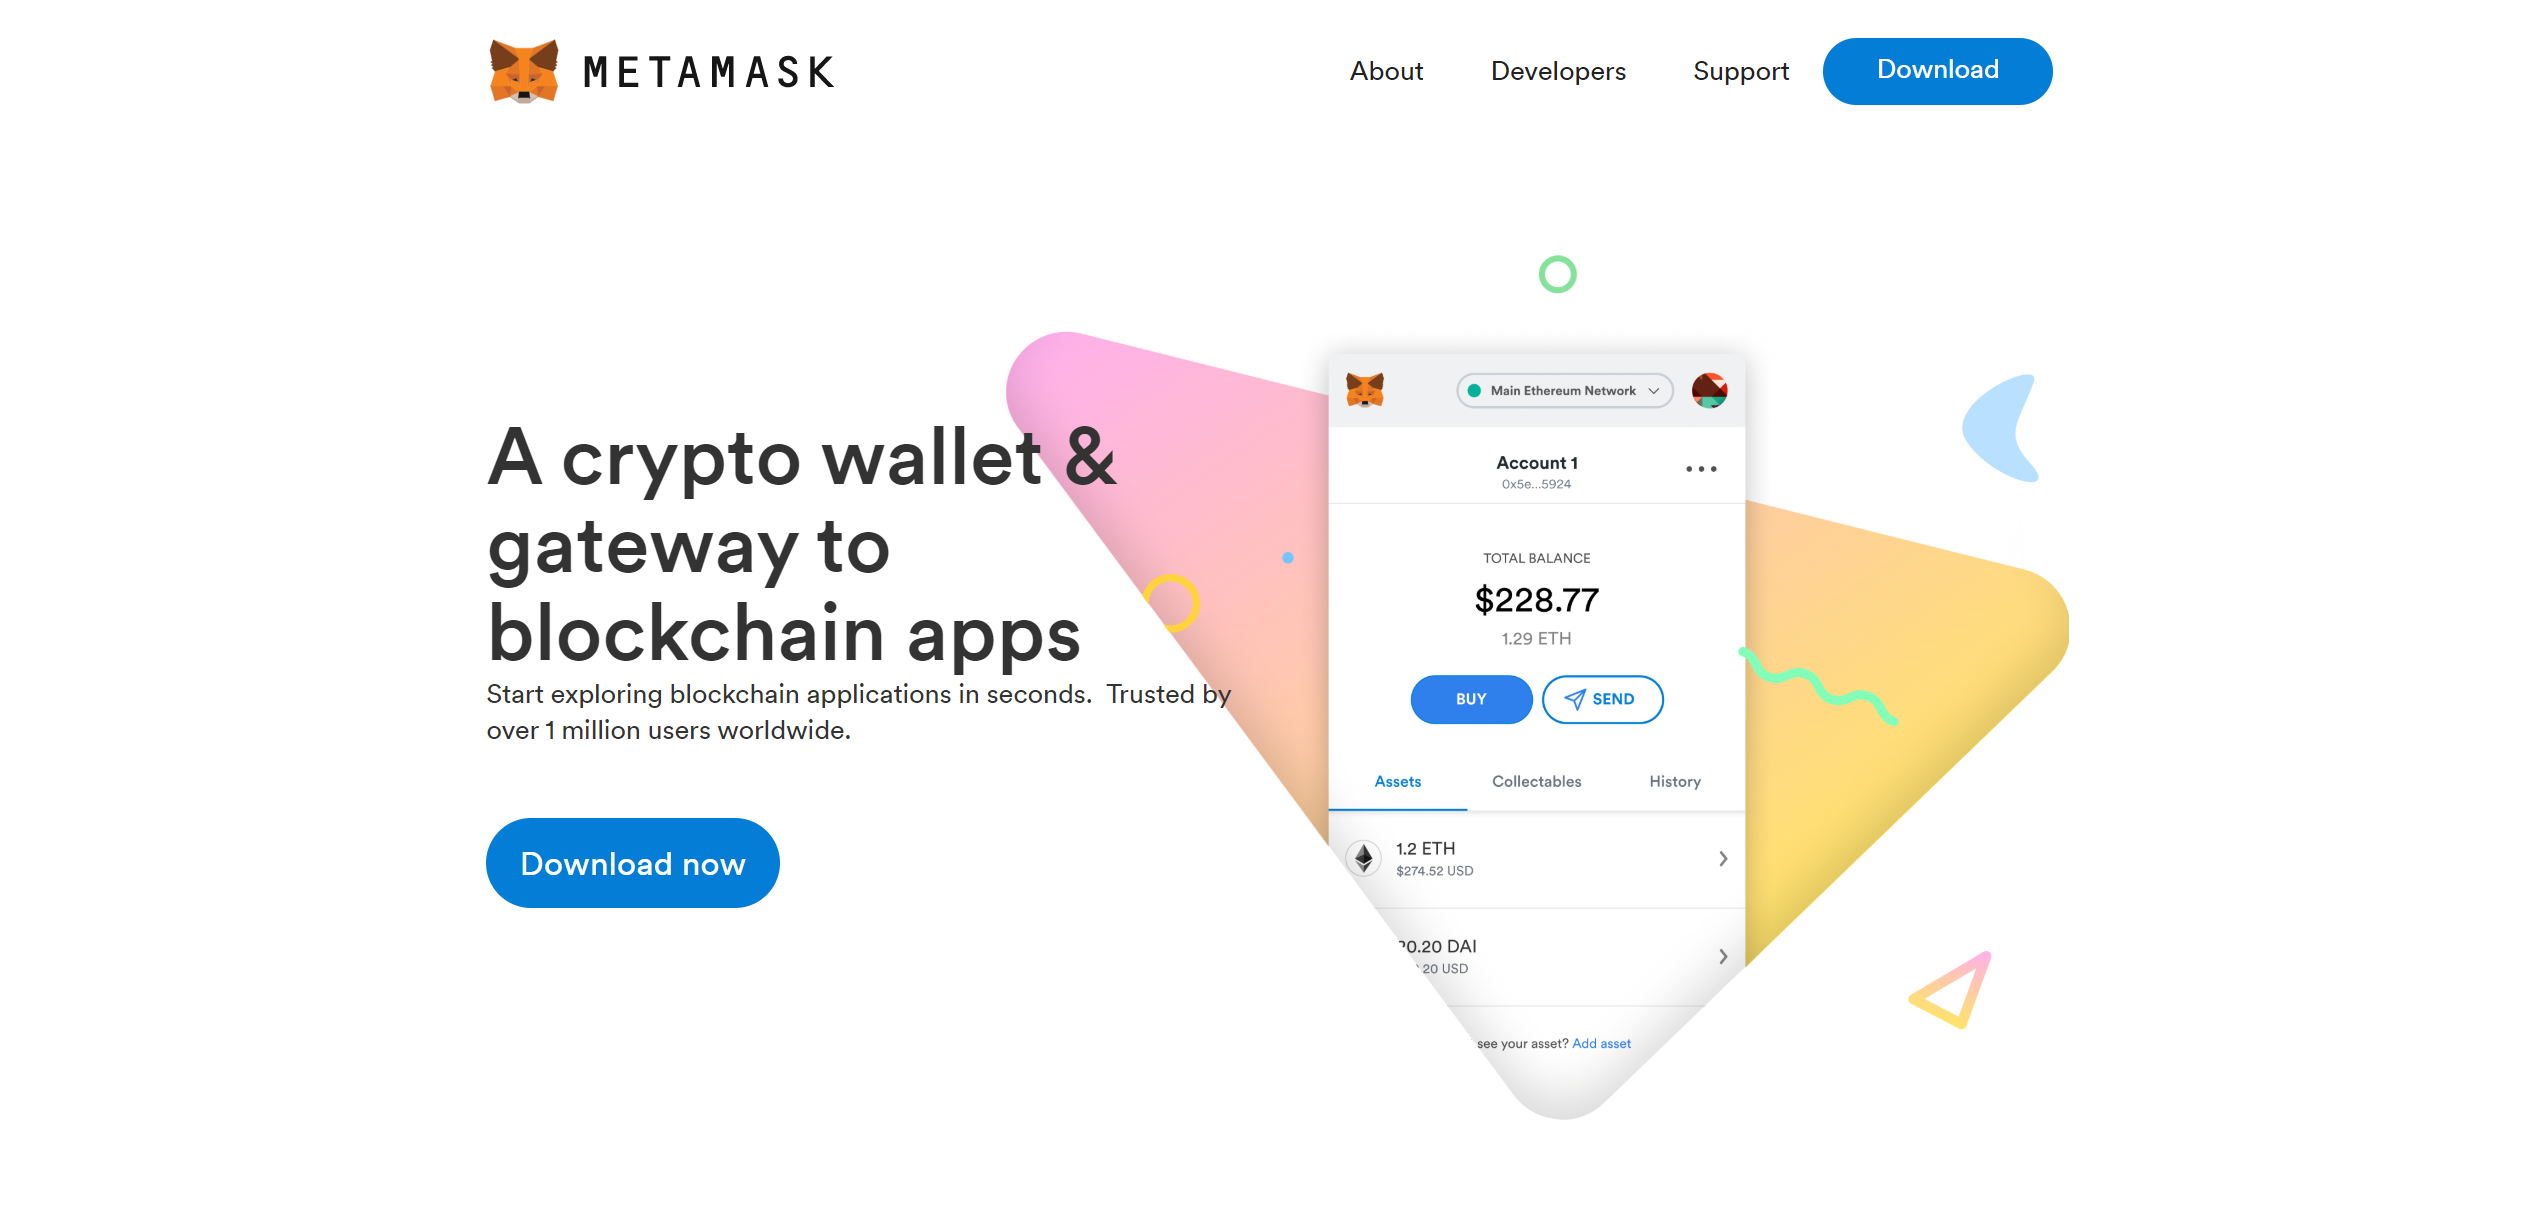
\includegraphics[width=\textwidth]{img/ch-wallets/metamask.png}
\end{borderbox}

\subsection[Hardware wallets]{Hardware wallets (cold)} 
\label{subsec:hardware-wallets}
Hardware wallets verschillen van software wallets in die zin dat de private keys van een gebruiker worden opgeslagen op een hardware apparaat zoals een USB. Hoewel hardware wallets transacties kunnen ondertekenen en versturen naar het netwerk, komt de private key nooit in directe verbinding met het internet, wat voor meer veiligheid zorgt. Hardware wallets ondersteunen meerdere cryptocurrencies, distributed ledger technologi{\"e}n, en communiceren met verschillende webinterfaces. Enkele goede wallets staan vermeld in \cref{tab:walletoverview}. Het uitvoeren van een transactie is eenvoudig. Gebruikers sluiten hun USB-apparaat aan op een computer of ander apparaat met internettoegang, voeren een pincode in, versturen de cryptocurrencies en bevestigen de transactie. 

 Een hardware wallet kan veilig en interactief worden gebruikt en private keys hoeven nooit in contact te komen met potentieel kwetsbare software of een online omgeving. Ten slotte is de software meestal open source, waardoor een gebruiker de volledige werking van het apparaat kan valideren.\medskip


\begin{tipbox}{\textbf{Tip}}
Bij een hardware wallet worden de private keys opgeslagen in een beschermde omgeving van de USB-stick en kunnen niet als tekst uit het apparaat worden ge{\"e}xporteerd. Daarnaast zijn hardware wallets immuun voor computervirussen.
\tcblower 
Gebruik een \href{https://shop.ledger.com/pages/ledger-nano-x?r=1849e3ffabd0}{Ledger} Hardware wallet.
\end{tipbox}

\medskip

\subsection{Paper wallets}{Paper wallets (cold)}
\label{subsec:paper-wallets}
Deze zijn eenvoudig te gebruiken en bieden een zeer hoge mate van veiligheid. Hoewel de term \say{papieren wallet} kan verwijzen naar een fysieke kopie of afdruk (op een stuk papier) van de public en private keys, kan het ook verwijzen naar een stuk software dat wordt gebruikt om keys te genereren die vervolgens veilig kunnen worden afgedrukt. Het overmaken van Bitcoin of een andere cryptocurrency naar een papieren wallet gebeurt door het overmaken van cryptocurrency van de software wallet naar het public address dat op de papieren wallet vermeld staat. Als je crypto wilt opnemen of uitgeven, hoef je alleen maar een transactie te sturen vanuit de papieren wallet naar de software wallet. Dit proces, dat vaak 'sweeping' wordt genoemd, kan handmatig worden uitgevoerd door het invoeren van de private-keys of door het scannen van de QR-code op de papieren wallet.

\medskip
\begin{borderbox}
    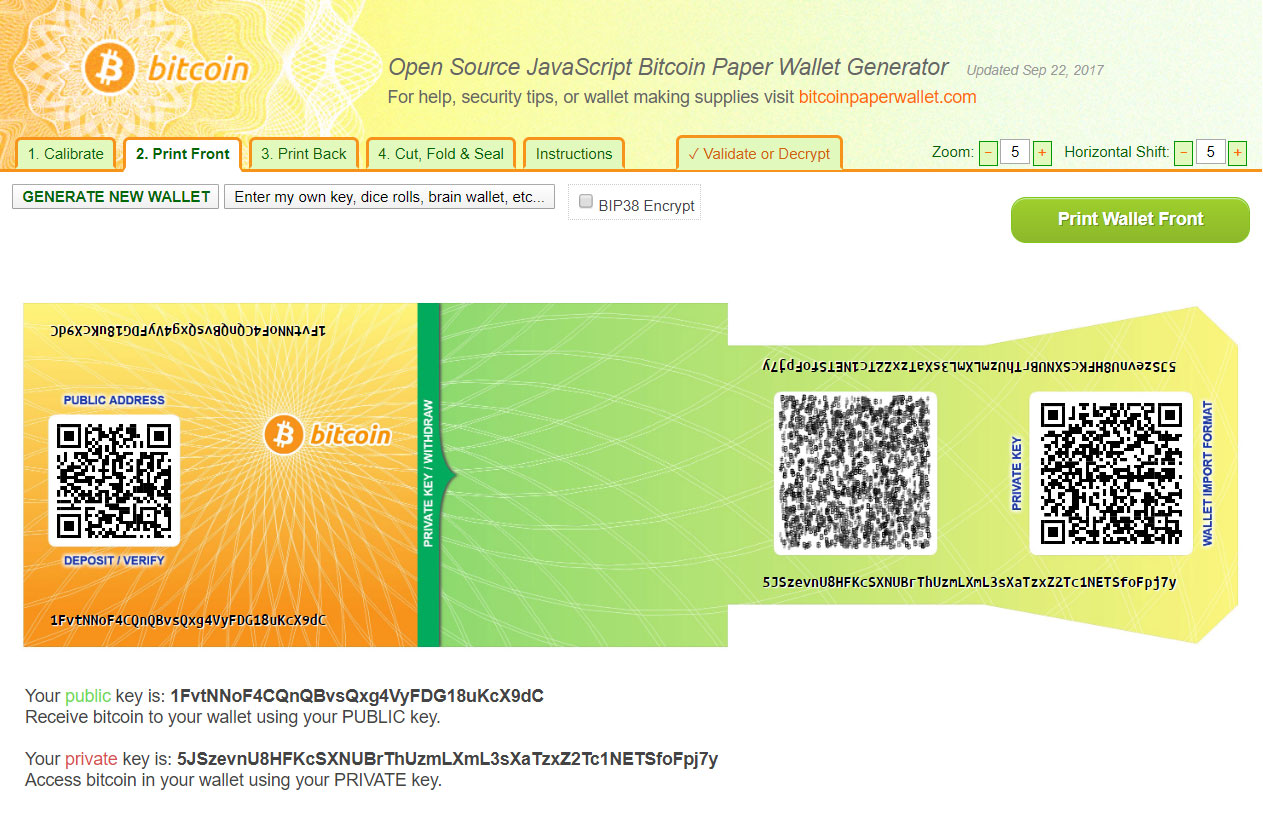
\includegraphics[width=\textwidth]{img/ch-wallets/paper-wallet-bitcoin.jpg}
\end{borderbox}
\medskip

Ondanks het feit dat papieren wallets veilig zijn, wordt het gebruik van deze wallets echter als gevaarlijk beschouwd en word het afgeraden om vaak te gebruiken. Een grote tekortkoming van paper wallets is dat ze niet geschikt zijn voor het versturen van een deel van het geld, maar slechts de hele balans in {\'e}{\'e}n keer.\medskip



\section{\emph{Best Practices} - crypto wallets}
Het is vrijwel altijd aangeraden potenti{\"e}le veiligheidsrisico's te beperken door je cryptocurrency te spreiden over verschillende wallets. Wie maar een relatief kleine som investeert, is waarschijnlijk ook met {\'e}{\'e}n wallet prima af. Gaat het om hogere bedragen, neem dan geen onnodige risico's en investeer in een hardware wallet (\cref{tab:walletoverview}). Daarnaast neem je wat cryptocurrency mee op een mobiele wallet. Het belangrijkste is dat je niet al je vermogen op {\'e}{\'e}n plaats bewaard, met crypto ben jij namelijk eindverantwoordelijk, niet de bank. \medskip

\begin{quotation}

      \textit{\say{Not your keys, not your Bitcoin.}}
      \begin{flushright}
        \small{--- \textbf{proofofkeys.com}}
      \end{flushright}
    
\end{quotation}

\subsection*{Een combinatie van wallets}
Probeer de potenti{\"e}le risico's te beperken door het vermogen te spreiden. Wanneer je diversifieert in meerdere cryptocurrencies met eigen doelen en ambities, spreidt je de risico's. Je kunt zowel binnen als buiten verschillende activas uitbreiden en diversifi{\"e}ren. Wanneer als het gaat om cryptocurrencies kan men bijvoorbeeld een deel van het vermogen meenemen op een mobiele wallet en de rest veilig opslaan op (meerdere) andere locaties.

Stel je deze situatie voor, je bent geregistreerd bij een broker exchange (om je fiat om te zetten in crypto) en bij een trading exchange (waar je crypto naar crypto handelt). Je hebt idealiter dan nog een speciale hardware wallet om het grootste deel van je activa offline op te slaan. Daarnaast download je een mobiele wallet om een klein deel op je telefoon mee te nemen om overal toegang te hebben en te kunnen besteden wanneer jij dit wilt. \medskip

\subsection*{Aanbevolen wallet configuratie}

Er zijn veel verschillende wallets beschikbaar en er worden regelmatig meer uiteenlopende en geavanceerde wallets gelanceerd. Voordat je een wallet selecteert, moet je goed nadenken over hoe je deze wilt gebruiken. Heb je een wallet nodig voor dagelijkse aankopen, of heb je een wallet nodig waar je actief mee kunt traden (handelen)? Heb je ook een speciale wallet nodig die fungeert als een offline kluis voor lange termijn investeringen? Ben je van plan om een groot aantal cryptocurrencies te gebruiken, of alleen Bitcoin en Ethereum? Heb je toegang tot jouw digitale wallet nodig vanaf meerdere apparaten of alleen vanaf je mobiele telefoon? Een selectie uitgelichte wallets staat in \cref{tab:walletoverview}. Wij adviseren op zijn minst een hardware wallet in combinatie een mobiele wallet, een desktop wallet, of een web wallet.\medskip


\begin{table}

\centering

\caption[Een selectie van cryptocurrency wallets]{Populaire cryptocurrency wallets in een overzicht. Web-hosted exchange wallets worden niet in overweging genomen, maar sommige van deze zijn gemarkeerd in \cref{ch:exchanges}.}
\begin{tabular}{llll} 
\toprule

\textbf{Wallet} & \textbf{Support} & \textbf{Platform} & \textbf{URL }\\
\midrule

Ledger          & multi    & hardware   & \href{https://shop.ledger.com/pages/ledger-nano-x?r=1849e3ffabd0}{ledger.com}\\
KeepKey         & multi    & hardware   & \href{http://lddy.no/aczp}{shapeshift.io}\\
Trezor          & multi    & hardware   & \href{https://shop.trezor.io/?offer_id=10&aff_id=3118}{trezor.io}\\
Electrum        & BTC      & desktop    & \href{https://electrum.org/#home}{electrum.org}\\
Atomic          & multi    & desktop    & \href{https://atomicwallet.io/}{atomicwallet.io}\\       
MEW             & ETH      & web        & \href{https://www.myetherwallet.com/}{myetherwallet.com}\\
MetaMask        & ETH      & web        & \href{https://metamask.io/}{metamask.io}\\
Exodus          & multi    & desktop    & \href{https://exodus.io/}{exodus.io}\\
Ethos           & multi    & mobiel     & \href{https://www.ethos.io/universal-wallet/}{ethos.io}\\
Abra            & multi    & mobiel     & \href{https://www.abra.com/}{abra.com}\\
Edge            & multi    & mobiel     & \href{https://edge.app/}{edge.app}\\
Changelly       & multi    & web        & \href{https://changelly.com/}{changelly.com}\\ 
ShapeShift      & multi    & web        & \href{https://shapeshift.com/#top}{shapeshift.com}\\

\bottomrule
\end{tabular}
\label{tab:walletoverview}
\end{table}


\subsection*{Wallet veiligheid}

Veiligheid van cryptocurrency wallets is een belangrijk onderwerp in de cryptocurrency wereld. Hoewel de meeste mensen niet bezig zijn met veiligheid, blijf het belangrijk om je bewust te zijn van de basis. Wanneer het fout gaat, is het vaak al te laat en zijn de wallet-gebruikers de dupe. Denk onder andere over de volgende dingen na: 

\begin{enumerate}[label=(\alph*)]
  \setlength\itemsep{0em}
    \item Partijen die veel gebruik maken van web wallets (hosted wallets) zijn meestal grote exchanges. Deze zijn mede hierdoor kwetsbaarder voor hacks en diefstal. Dit is in het verleden al geregeld gebeurt en er is veel informatie beschikbaar over het verlies van cryptocurrencies van duizenden gebruikers als gevolg van grootschalige veiligheids compromissen. 
    \item Veel gecentraliseerde partijen en exchanges de controle over de private-keys uit handen gegeven. In plaats daarvan kun je bij deze exchanges inloggen met een combinatie van gebruikersnaam en wachtwoord.
    \item Dit houdt in dat je niet in de volledige controle behoudt over jouw eigen vermogen, aangezien de exchange je private key in handen heeft.
    \item Overweeg het gebruik van meerdere wallets, en bewaar het meerendeel van jouw cryptocurrency via een hardware wallet - in cold storage.
\end{enumerate}

\medskip

\subsection*{Geavanceerde wallets}

Houd er rekening mee dat aan een beter beveiligde wallet meerdere lagen technologie worden toegevoegd. Deze technologische complexiteit brengt ook extra risico's met zich mee voor gebruikers als ze niet precies weten hoe ze deze wallets moeten gebruiken. Beoordeel dus zelf wat een aanvaardbaar risiconiveau is voor jouw specifieke situatie en omstandigheden, gebaseerd op je eigen kennis, en op basis van je totale inleg en ge{\"i}nvesteerde middelen.
Het is gemakkelijker om een wallet op je telefoon of desktop te installeren, waar dan ingelogd kan worden via een eenvoudige PIN-code of wachtwoord. Een complexere wallet zoals een cold storage of multi-signature wallet staat niet meteen gelijk aan een algehele betere beveiliging. De beveiliging is namelijk maar zo goed als de gebruiker de juiste kennis correct toepast. Beter beveiligde cryptocurrency wallets - en de vrijheid en verantwoordelijkheid die deze met zich mee brengen - vragen over het algemeen dus meer kennis van de gebruiker. 






